\documentclass[11pt,a4paper]{article}
\usepackage[utf8]{inputenc}
\usepackage[margin=1in]{geometry}
\usepackage{graphicx}
\usepackage{hyperref}
\usepackage{listings}
\usepackage{xcolor}
\usepackage{titlesec}
\usepackage{enumitem}
\usepackage{booktabs}
\usepackage{fancyhdr}

% Custom Colors
\definecolor{primaryblue}{RGB}{37, 99, 235}
\definecolor{codegreen}{rgb}{0,0.6,0}
\definecolor{codegray}{rgb}{0.5,0.5,0.5}
\definecolor{codepurple}{rgb}{0.58,0,0.82}
\definecolor{backcolour}{rgb}{0.95,0.95,0.92}

% Code Style
\lstdefinestyle{mystyle}{
    backgroundcolor=\color{backcolour},   
    commentstyle=\color{codegreen},
    keywordstyle=\color{magenta},
    numberstyle=\tiny\color{codegray},
    stringstyle=\color{codepurple},
    basicstyle=\ttfamily\footnotesize,
    breakatwhitespace=false,         
    breaklines=true,                 
    captionpos=b,                    
    keepspaces=true,                 
    numbers=left,                    
    numbersep=5pt,                  
    showspaces=false,                
    showstringspaces=false,
    showtabs=false,                  
    tabsize=2
}
\lstset{style=mystyle}

% Header/Footer
\pagestyle{fancy}
\fancyhf{}
\rhead{Atharva M. \& Harshita G.}
\lhead{Notes App Project}
\rfoot{Page \thepage}

\begin{document}

% --- TITLE PAGE ---
\begin{titlepage}
    \centering
    \vspace*{2cm}
    {\Huge \textbf{Minimalist Full-Stack}}\\[0.5cm]
    {\Huge \textbf{Notes Application}}\\[1cm]
    {\Large Semester Project | Web Programming Lab}\\[2cm]
    
    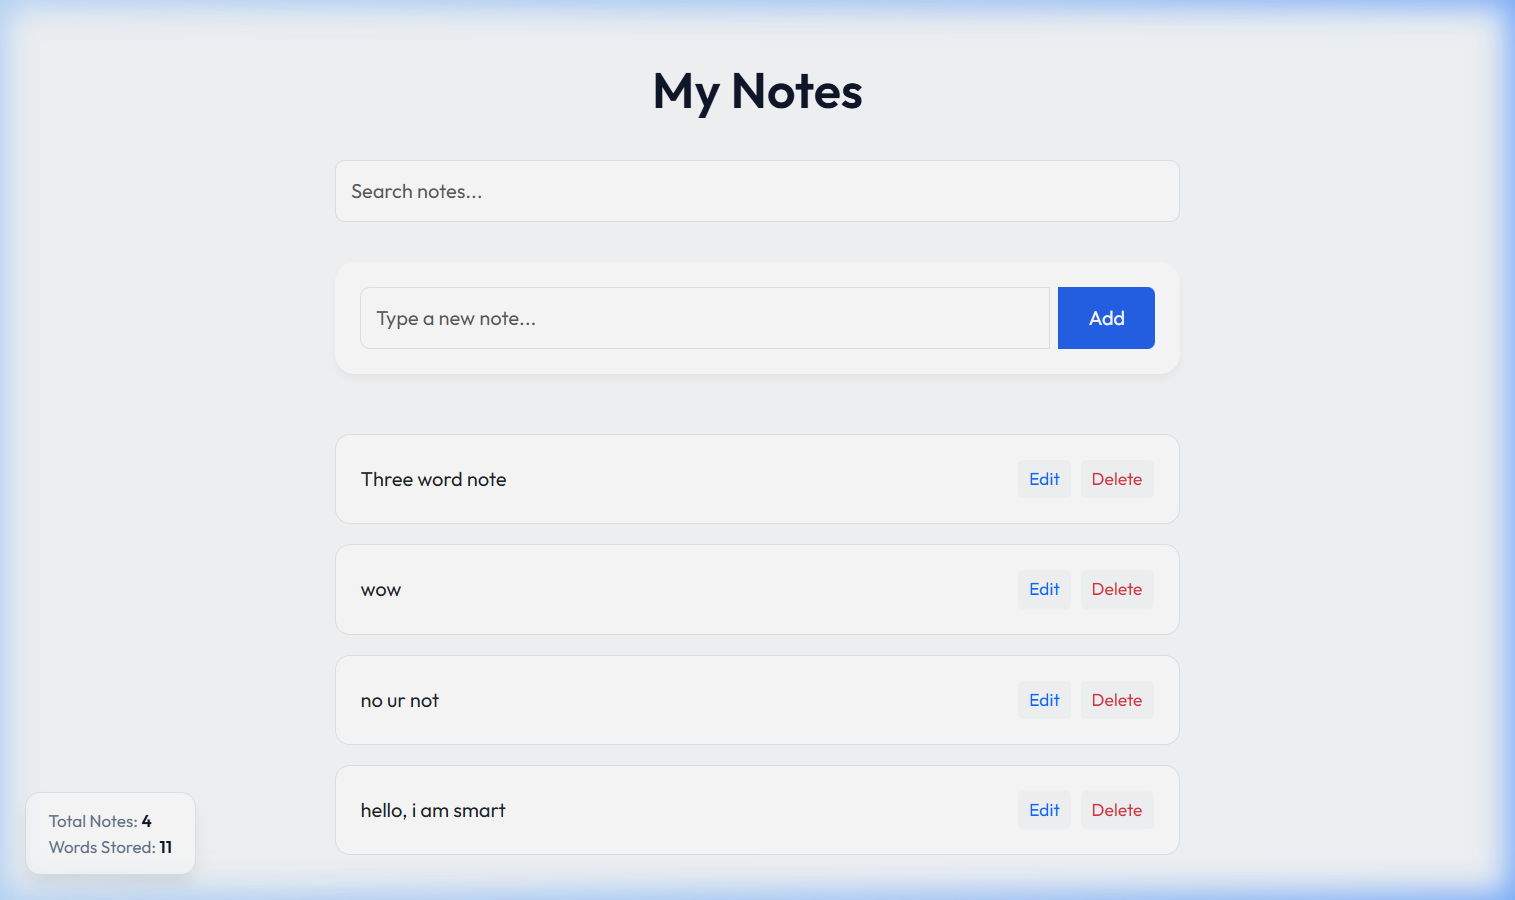
\includegraphics[width=0.85\textwidth]{main_app.png}\\[2cm]
    
    {\large \textbf{SUBMITTED BY:}}\\[0.5cm]
    {\large \textbf{Atharva Maikhuri} (235816206)}\\
    {\large \textbf{Harshita Gaurav} (235816036)}\\[2cm]
    
    {\large April 14, 2026}\\[1cm]
    {\large \textbf{DEPARTMENT OF COMPUTER APPLICATIONS}}
\end{titlepage}

\newpage
\tableofcontents

\newpage
\section{Project Objective and Scope}
The core objective of this project is to develop a lightweight, user-friendly, and highly interactive Note-Taking web application. It serves as a comprehensive demonstration of Full-Stack development concepts, focusing on the seamless integration of a Python-based backend (Django) with a dynamic JavaScript frontend (jQuery \& AJAX).
The project scope encompasses real-time data management through a RESTful architecture, ensuring a smooth user experience that mirrors modern Single-Page Applications (SPAs).

\section{Design Philosophy: The Power of Minimalism}
In modern web development, ``Minimalism'' is not just an aesthetic choice but a usability priority. This application was designed to reduce cognitive load by focusing on core functionality while ensuring high-quality interactions. By avoiding the common ``purple'' color palettes of generic templates and opting for a professional Azure/Slate theme, we created a tool that feels focused and purpose-built.

\newpage
\section{Detailed Technology Stack}
This project utilizes a curated stack designed for performance and rapid development.
\begin{itemize}
    \item \textbf{Backend: Django Ecosystem}: Django provides a high-security environment with an integrated Object-Relational Mapper (ORM).
    \item \textbf{Frontend: Bootstrap 5 \& jQuery}: Provides a flexible grid system and efficient handling of AJAX requests.
    \item \textbf{Database: SQLite}: Managed via the Django ORM to provide a zero-configuration storage engine.
\end{itemize}

\section{Scalability and Efficiency}
The system is designed with scalability in mind. The Django ORM allows for a transition to enterprise-grade databases like PostgreSQL without changing business logic. The client-side search filtering is optimized to handle hundreds of notes with minimal latency.

\newpage
\section{System Architecture}
The application follows the Model-View-Template (MVT) design pattern, ensuring a clean separation of data, logic, and presentation.

\begin{figure}[h]
    \centering
    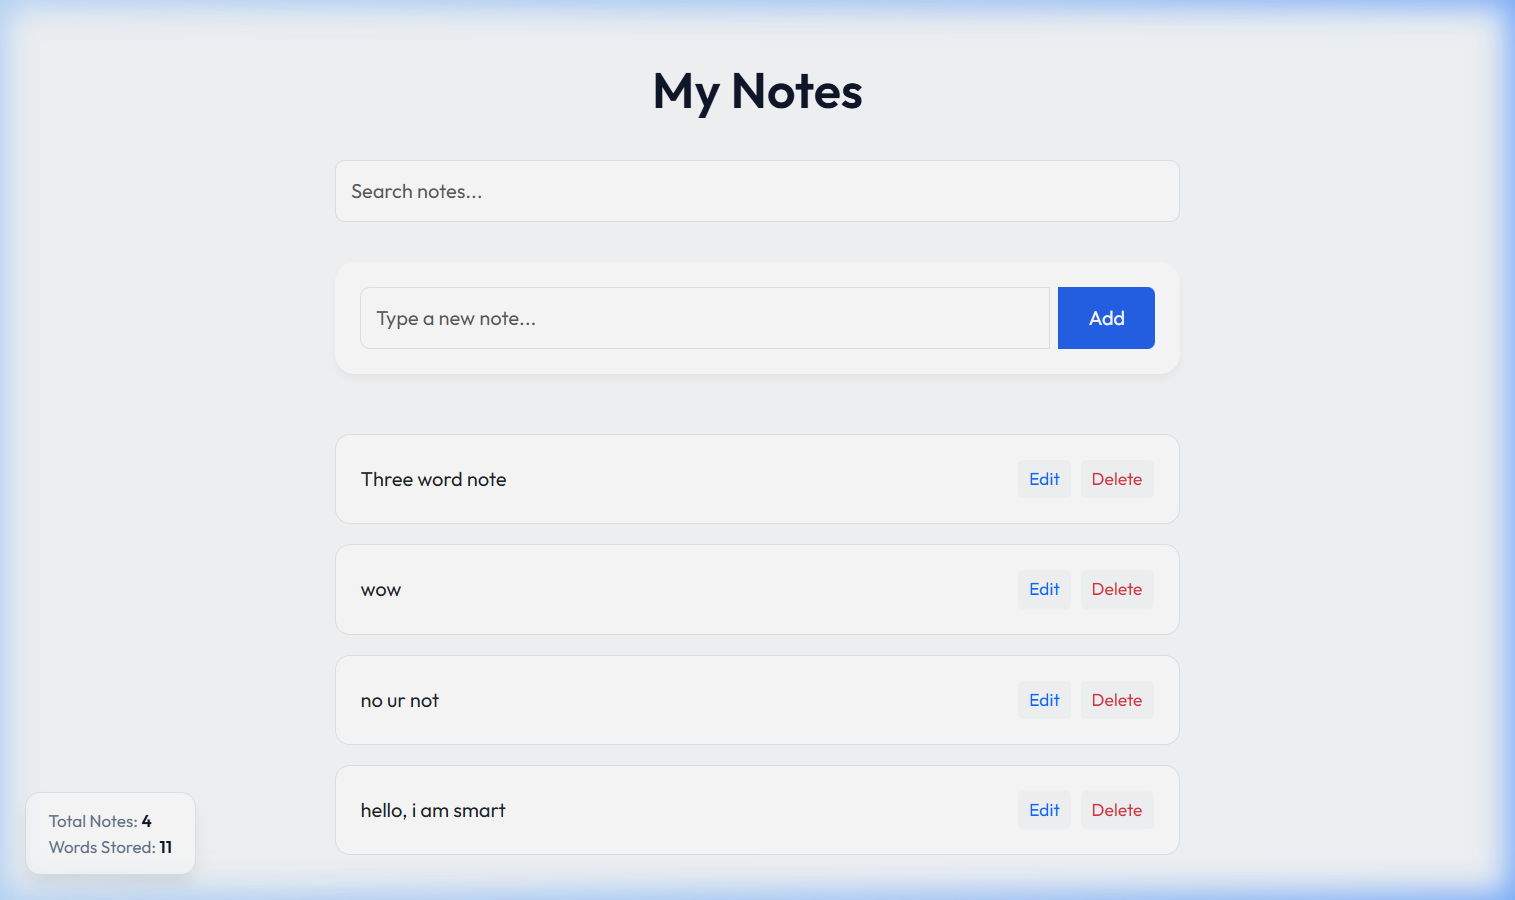
\includegraphics[width=0.75\textwidth]{main_app.png}
    \caption{Main Dashboard showing clean statistics and asynchronous notes list.}
\end{figure}

\subsection{Request Lifecycle (The AJAX Loop)}
Every dynamic update in the app follows a high-speed lifecycle where jQuery stops the page reload, sends an AJAX POST request, Django processes it, and the server returns a success signal.

\newpage
\section{Security and Input Integrity}
\subsection{CSRF Protection in AJAX}
To prevent Cross-Site Request Forgery, state-changing requests include CSRF tokens. This is handled dynamically by extracting the cookie or using injected headers.

\subsection{Real-time Form Validation}
Invalid data is blocked before reaching the server, providing the user with an intuitive experience.
\begin{figure}[h]
    \centering
    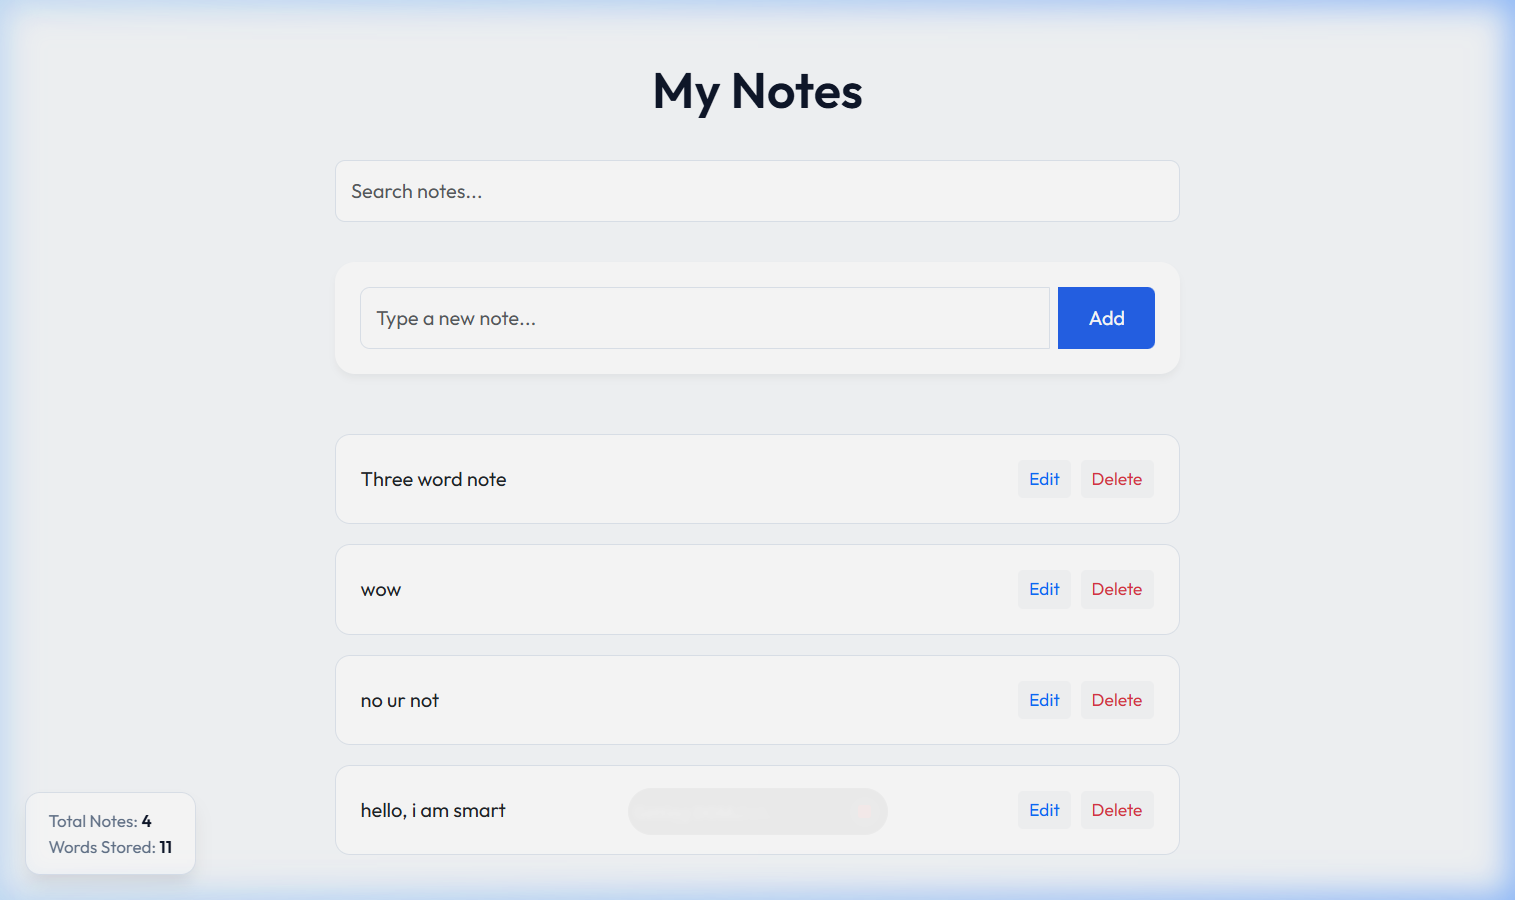
\includegraphics[width=0.6\textwidth]{validation_error.png}
    \caption{Dynamic validation preventing empty entries.}
\end{figure}

\newpage
\section{RESTful API Reference}
\begin{table}[h]
    \centering
    \begin{tabular}{@{}llll@{}}
        \toprule
        \textbf{Method} & \textbf{URL} & \textbf{Function} \\ \midrule
        GET & /api/notes/ & Fetch latest notes. \\
        POST & /api/add/ & Add a new note. \\
        POST & /api/update/<id>/ & Update content. \\
        DELETE & /api/delete/<id>/ & Remove permanently. \\ \bottomrule
    \end{tabular}
\end{table}

\section{Dynamic Modals \& Maintenance}
Bootstrap Modals ensure a focused editing experience. The code's modular structure allows for easy future extensions like Category or Priority fields.
\begin{figure}[h]
    \centering
    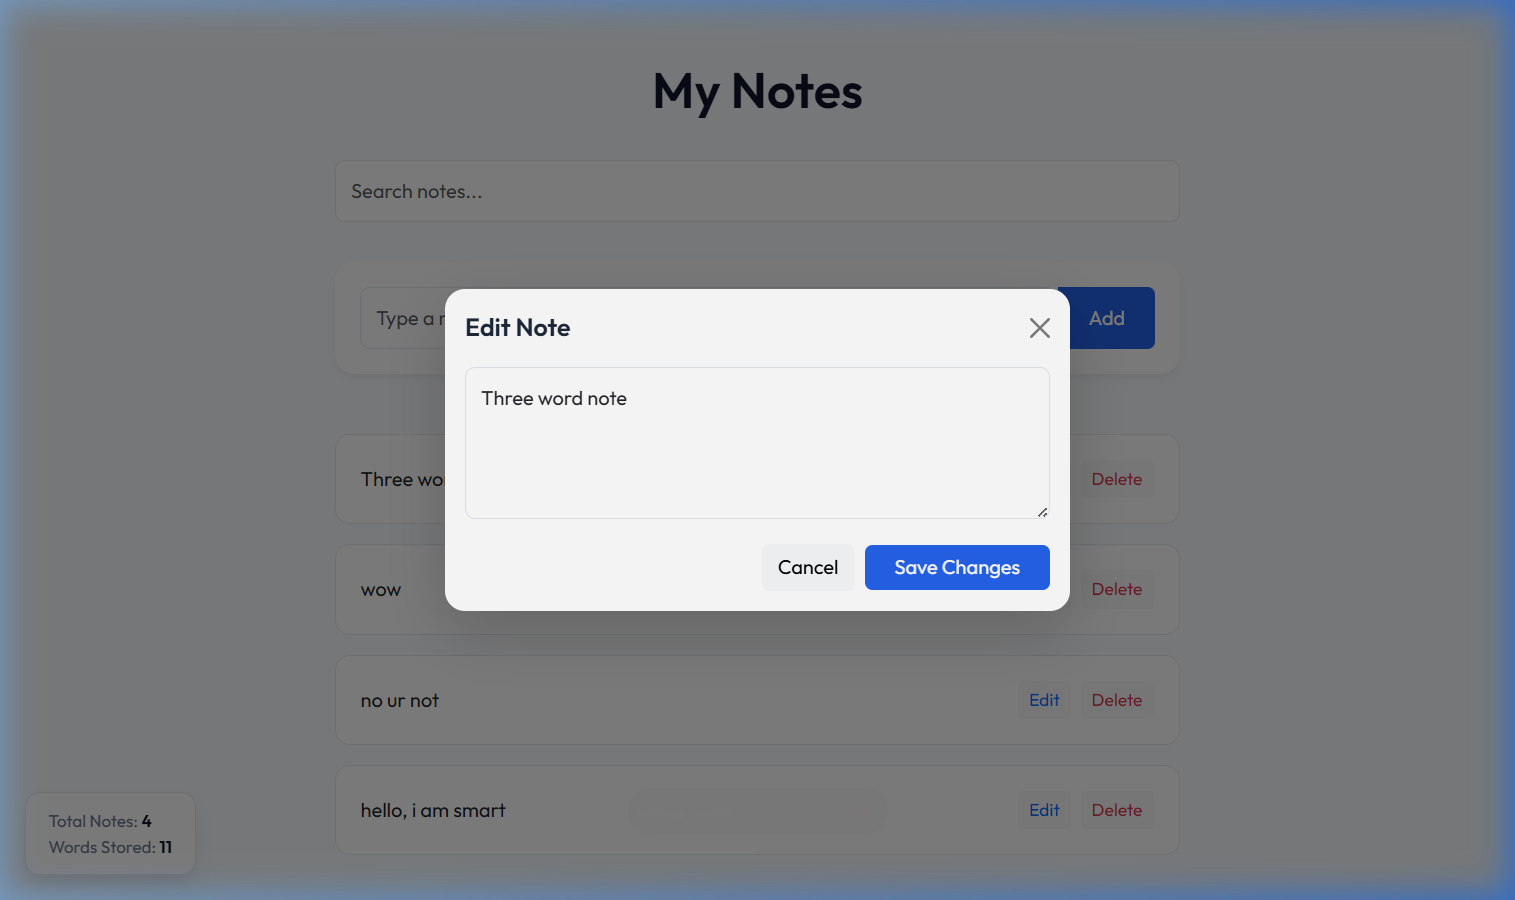
\includegraphics[width=0.6\textwidth]{edit_modal.png}
    \caption{The Edit Modal centered on the viewport.}
\end{figure}

\newpage
\section{Conclusion}
The Minimalist Notes Application successfully fulfills all requirements. By bridging the gap between Python server-side strengths and JavaScript frontend agility, we produced a modern, sleek, and functional application.

\begin{center}
    \vspace{2cm}
    \textbf{END OF PROJECT REPORT}\\
    Atharva Maikhuri (235816206) | Harshita Gaurav (235816036)\\
    April 14, 2026
\end{center}

\end{document}
